\documentclass[12pt]{article}

\usepackage[margin=1in]{geometry}
\usepackage{graphicx}

\title{Basic Forest Fire Information}
\author{Corwin de Boor}

\begin{document}
\maketitle

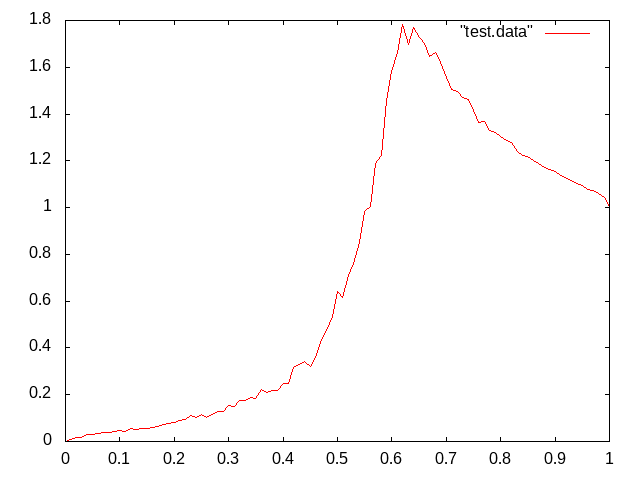
\includegraphics[height=2in]{basicfire}

\begin{description}
	\item[Grid Size] $100\times100$
	\item[Trials] $100$
	\item[Resolution] $0.01$ between each point
	\item[Peak] $64\%$ trees $1.785$ time
\end{description}

When the graph is very sparse, the fire burns out before it can reach many of
the trees. As more trees are added, the fire is able to burn all of them
down, but not in an easy linear fashion. When even more trees are added, they
become close enough that they are able to burn in a quick and linear fashion,
without much backtracking. That causes the sharp increase and then decline.

\end{document}
